\documentclass[12pt]{article}

\usepackage[utf8x]{inputenc}
\usepackage[english]{babel}
\usepackage{subcaption}
\usepackage{amssymb,amsmath,amsthm,amsfonts}
\usepackage{calc}
\usepackage{graphicx}
\usepackage[shortlabels]{enumitem}
\usepackage{gensymb}
\usepackage{float}
\usepackage{natbib}
\usepackage{url}
\usepackage[utf8x]{inputenc}
\usepackage{amsmath}
\usepackage{graphicx}
\graphicspath{{images/}}
\usepackage{parskip}
\usepackage{fancyhdr}
\usepackage{vmargin}
\usepackage{mathrsfs}
\usepackage[dvipsnames]{xcolor}
\usepackage{longtable}
\usepackage{multicol}
\usepackage{multirow}
\usepackage{booktabs}

%tikzpicture
\usepackage{tikz}
\usepackage{scalerel}
\usepackage{pict2e}
\usepackage{tkz-euclide}
\usetikzlibrary{calc}
\usetikzlibrary{patterns,arrows.meta}
\usetikzlibrary{shadows}
\usetikzlibrary{external}
\usepackage{listings}
\usepackage{xcolor}


\definecolor{lightgray}{rgb}{0.95,0.95,0.95}  % gris muy claro
% más oscuro:
% \definecolor{lightgray}{rgb}{0.9,0.9,0.9}
% aún más plomo:
% \definecolor{lightgray}{rgb}{0.85,0.85,0.85}

\lstset{
    language=C,
    basicstyle=\ttfamily\small,
    keywordstyle=\color{blue},
    commentstyle=\color{green!50!black},
    stringstyle=\color{red},
    numbers=left,
    numberstyle=\tiny,
    stepnumber=1,
    numbersep=5pt,
    frame=single,
    breaklines=true,
    tabsize=2
}
%pgfplots
\usepackage{pgfplots}
\pgfplotsset{compat=newest}
\usepgfplotslibrary{statistics}
\usepgfplotslibrary{fillbetween}

\setmarginsrb{3 cm}{2.5 cm}{3 cm}{2.5 cm}{1 cm}{1.5 cm}{1 cm}{1.5 cm}

\title{Homework 3}					% Titulo
\author{Matías I. Inostroza (mii2106)}					% Autor
\date{\today}						% Fecha


\makeatletter
\let\thetitle\@title
\let\theauthor\@author
\let\thedate\@date
\makeatother

\pagestyle{fancy}
\fancyhf{}
\rhead{\theauthor}
\lhead{\thetitle}
\cfoot{\thepage}

\begin{document}

%%%%%%%%%%%%%%%%%%%%%%%%%%%%%%%%%%%%%%%%%%%%%%%%%%%%%%%%%%%%%%%%%%%%%%%%%%%%%%%%%%%%%%%%%

\begin{titlepage}
	\centering
    \vspace*{0.0 cm}
    
\includegraphics[scale = 0.35]{Columbia_logo.png}\\[2.0 cm]	% Logo Universidad
    \textsc{\LARGE Columbia University}\\[2.0 cm]	% Nombre Universidad
	\textsc{\Large APMAE4302}\\[0.5 cm]				% Codigo Curso
	\textsc{\large Methods in computational science}\\[0.5 cm]		% Nombre Curso
	\rule{\linewidth}{0.2 mm} \\[0.4 cm]
	{ \huge \bfseries \thetitle}\\
	\rule{\linewidth}{0.2 mm} \\[1.5 cm]
	
	\begin{minipage}{0.4\textwidth}
		\begin{center} \large
			\emph{Author:}\\
			\theauthor\linebreak
			\end{center}
	\end{minipage}\\[2 cm]
	
	{March 9, 2026}\\[2 cm]
 
	\vfill
	
\end{titlepage}

%%%%%%%%%%%%%%%%%%%%%%%%%%%%%%%%%%%%%%%%%%%%%%%%%%%%%%%%%%%%%%%%%%%%%%%%%%%%%%%%%%%%%%%%%


\pagebreak

%%%%%%%%%%%%%%%%%%%%%%%%%%%%%%%%%%%%%%%%%%%%%%%%%%%%%%%%%%%%%%%%%%%%%%%%%%%%%%%%%%%%%%%%%
\section{Problem 1}

\textbf{1)} First, the $f$ function is needed. For find it, the following exact solution is given $u_{exact}(x,y)$ 
\begin{equation}
    u_{exact}(x,y)= A \exp\left(-\frac{(x-x_0)^2+(y-y_0)^2}{\sigma^2}\right)
\end{equation}

Setting $b =\left(-\frac{(x-x_0)^2+(y-y_0)^2}{\sigma^2}\right) \rightarrow u_{exact} = A\exp(b)$

\begin{itemize}
    \item $\frac{\partial u}{\partial x} = A\exp(b)\frac{\partial b}{\partial x}$
    \item $\frac{\partial^2 u}{\partial x^2} = A\left[\exp(b)\left(\frac{\partial b}{\partial x}\right)^2 + \exp(b)\frac{\partial^2 b}{\partial x^2}\right] = A\exp(b)\left[\left(\frac{\partial b}{\partial x}\right)^2 + \frac{\partial^2 b}{\partial x^2}\right] $
    \item $\frac{\partial u}{\partial y} = A\exp(b)\frac{\partial b}{\partial y}$
    \item $\frac{\partial^2 u}{\partial y^2} = A\left[\exp(b)\left(\frac{\partial b}{\partial y}\right)^2 + \exp(b)\frac{\partial^2 b}{\partial y^2}\right] = A\exp(b)\left[\left(\frac{\partial b}{\partial y}\right)^2 +\frac{\partial^2 b}{\partial y^2}\right]$
\end{itemize}

Then, the equation is:

\begin{eqnarray}
    -\left(A\exp(b)\left[\left(\frac{\partial b}{\partial x}\right)^2 + \frac{\partial^2 b}{\partial x^2}\right] +  A\exp(b)\left[\left(\frac{\partial b}{\partial y}\right)^2 +\frac{\partial^2 b}{\partial y^2}\right] \right) + \gamma \left(A\exp(b)\right)^p = f\\
    -A\exp(b)\left(\left(\frac{\partial b}{\partial x}\right)^2 + \left(\frac{\partial b}{\partial y}\right)^2 + \frac{\partial^2 b}{\partial x^2}  +\frac{\partial^2 b}{\partial y^2} \right) + \gamma \left(A\exp(b)\right)^p = f
\end{eqnarray}

And $\frac{\partial b}{\partial x} = -\frac{2(x-x_0)}{\sigma^2}$, $\frac{\partial^2 b}{\partial x^2} = -\frac{2}{\sigma^2}$, $\frac{\partial b}{\partial y} = -\frac{2(y-y_0)}{\sigma^2}$, $\frac{\partial^2 b}{\partial y^2} = -\frac{2}{\sigma^2}$

\begin{eqnarray}
    -A\exp(b)\left(\frac{4}{\sigma^4}((x-x_0)^2 + (y-y_0)^2) - \frac{4}{\sigma^2}\right) + \gamma \left(A\exp(b)\right)^p = f\\
    -A\exp(b)\left(-\frac{2}{\sigma^2}b - \frac{4}{\sigma^2}\right) + \gamma \left(A\exp(b)\right)^p = f \\
    \frac{2}{\sigma^2}A\exp(b)\left( b + 2\right) + \gamma \left(A\exp(b)\right)^p = f
\end{eqnarray}

The discretization  is the following:

\begin{eqnarray}
\frac{\partial^2 u}{\partial x^2} \approx \frac{u^{i-1,j} - 2u^{i,j} + u^{i+1,j}}{\Delta x^2} \\
\frac{\partial^2 u}{\partial y^2} \approx \frac{u^{i,j-1} - 2u^{i,j} + u^{i,j+1}}{\Delta y^2} 
\end{eqnarray}

So that, the equation is:

\begin{equation}
  - \frac{u^{i-1,j} - 2u^{i,j} + u^{i+1,j}}{\Delta x^2} - \frac{u^{i,j-1} - 2u^{i,j} + u^{i,j+1}}{\Delta y^2} + \gamma (u^{i,j})^p = f
\end{equation}

If the grid is equally spaced, that means $\Delta x = \Delta y = h$:

\begin{equation}
      \frac{ 4u^{i,j} -u^{i-1,j} - u^{i+1,j} - u^{i,j-1}- u^{i,j+1}}{h^2} + \gamma (u^{i,j})^p = f  
\end{equation}

So that the residual is:

\begin{equation}
      F^{i,j}(u) =    \frac{ 4u^{i,j} -u^{i-1,j} - u^{i+1,j} - u^{i,j-1}- u^{i,j+1}}{h^2} + \gamma (u^{i,j})^p - f = 0  
\end{equation}

And for the boundary nodes:

\begin{equation}
    F^{i,j}(u) = u^{i,j} - u_{exact}(x_i,y_i) = 0
\end{equation}

\textbf{2)} The Jacobian corresponds to the equation's derivatives with respect to the $u$ variables. For nodes that are inside the grid:

\begin{eqnarray}
    \frac{\partial F^{i,j}}{\partial u^{i,j}} = \frac{4}{h^2} + \gamma p (u^{i,j})^{p-1}\\
    \frac{\partial F^{i,j}}{\partial u^{i+1,j}} = \frac{\partial F^{i,j}}{\partial u^{i-1,j}} = \frac{\partial F^{i,j}}{\partial u^{i,j+1}} = \frac{\partial F^{i,j}}{\partial u^{i,j-1}} = -\frac{1}{h^2}
\end{eqnarray}

And for the boundary:

\begin{equation}
    \frac{\partial F^{i,j}}{\partial u^{i,j}} = 1
\end{equation}
\begin{equation}
    J(u) = 1
\end{equation}
If all unknowns are stacked into a global vector $\mathbf{u}$, the Jacobian for the interior equations can be written as
\begin{equation}
\mathbf{J}(\mathbf{u}) = \mathbf{A} + \gamma p \, \mathrm{diag}\!\left(\mathbf{u}^{[p-1]}\right),
\end{equation}
where $\mathbf{A}$ is the five point finite difference matrix associated with the operator $-\nabla^2$ (each row as $\begin{bmatrix} ...& -1 & ...&-1&4&-1&...&-1&...
    \end{bmatrix} $), and $\mathrm{diag}(\mathbf{u}^{[p-1]})$ is a diagonal matrix whose entries are $u_k^{p-1}$.

For boundary nodes, the corresponding rows of the Jacobian are replaced by rows of the identity matrix, since the boundary residual is simply $u_k-g_k=0$.
Thus, the global Jacobian is obtained by using the interior stencil rows for interior nodes and identity rows for boundary nodes.

\textbf{3)} 

\textbf{ a)} For this problem, the code \texttt{reaction2d.c} was wrote and attached and uploaded to the repositori


\textbf{ b)}The function $f$ is controlled to be $f = -\nabla^2u_{exact}$ when \texttt{-rct\_linear\_f} is set, and  $f = -\nabla^2u_{exact} + \gamma u^p$ as the following piece of code

\begin{lstlisting}
PetscReal fRHS(PetscReal x, PetscReal y, AppCtx *user) {
    PetscReal f = -d2ufunction(x,y);
    if (!user->linear_f) {
        PetscReal uex = ufunction(x, y);
        f += user->gamma * PetscPowReal(uex, (PetscReal)user->p);
    }
    return f;
\end{lstlisting}

\textbf{ c)} For the residual is created from the function:
\begin{lstlisting}
PetscErrorCode FormFunctionLocal(DMDALocalInfo *info,
                                 PetscReal **u,
                                 PetscReal **FF,
                                 AppCtx    *user) {
                                 .
                                 .
                                 .
                                 }
\end{lstlisting}

And the jacobian by the function:

\begin{lstlisting}
PetscErrorCode FormJacobianLocal(DMDALocalInfo *info,
                                 PetscReal    **u,
                                 Mat           J,
                                 Mat           P,
                                 AppCtx       *user) {
                                 .
                                 .
                                 .
                                 }
\end{lstlisting}

\textbf{d)} The code can set the Jacobian option through the lines

\begin{lstlisting}
    PetscCall(DMDASNESSetJacobianLocal(da,
              (DMDASNESJacobianFn *)FormJacobianLocal, &user));
    PetscCall(SNESSetFromOptions(snes));
\end{lstlisting}

The call to \texttt{SNESSetFromOptions} allows PETSc to override the analytical Jacobian registered in \texttt{DMDASNESSetJacobianLocal} with finite-difference approximations using the options -snes\_fd, -snes\_fd\_color, -snes\_mf, and -snes\_mf\_operator at runtime, without modifying the code.

\textbf{e)} Paraview option is set by the following lines:

\begin{lstlisting}
    PetscCall(PetscViewerVTKOpen(PETSC_COMM_WORLD, "reaction2d.vtr",
                                 FILE_MODE_WRITE, &viewer));
    PetscCall(PetscObjectSetName((PetscObject)u,      "u"));
    PetscCall(PetscObjectSetName((PetscObject)uexact, "uexact"));
    PetscCall(VecView(u,      viewer));
    PetscCall(VecView(uexact, viewer));
    PetscCall(DMView(da,      viewer));
    PetscCall(PetscViewerDestroy(&viewer));
\end{lstlisting}

The variable $u$ is the solution from finite difference method, and $uexact$ is the exact solution. There is no RHS output because in Newton Raphson there is no RHS but residual evaluations. Note that this was extracted from \texttt{poisson2d.c} code

\textbf{4)} For a  $65\times65$ grid with $\gamma$, the following result is obtained:

\begin{lstlisting}
  0 SNES Function norm 7.337078385146e+02
    0 KSP Residual norm 7.337078385146e+02
    1 KSP Residual norm 6.204150044152e-11
  1 SNES Function norm 6.379557175902e-11
on 65 x 65 grid:  rel_error |u-uexact|_2/|uexact|_2 = 0.000524515
\end{lstlisting}

The method converges in one iteration of the Newton Raphson method with a $\|F(u)\|_2 = 6.38\times10^{-11}<10^{-10}$ and a relative error of $5.24\times10^{-4}$. The linear system at each Newton step was solved using direct LU factorization with \texttt{-ksp\_type preonly -pc\_type lu -pc\_factor\_mat\_solver\_type mumps}, converging in 1 KSP iteration (see \texttt{options\_file\_gamma0} in files at the HW3 folder)

\begin{figure}[h]
\centering
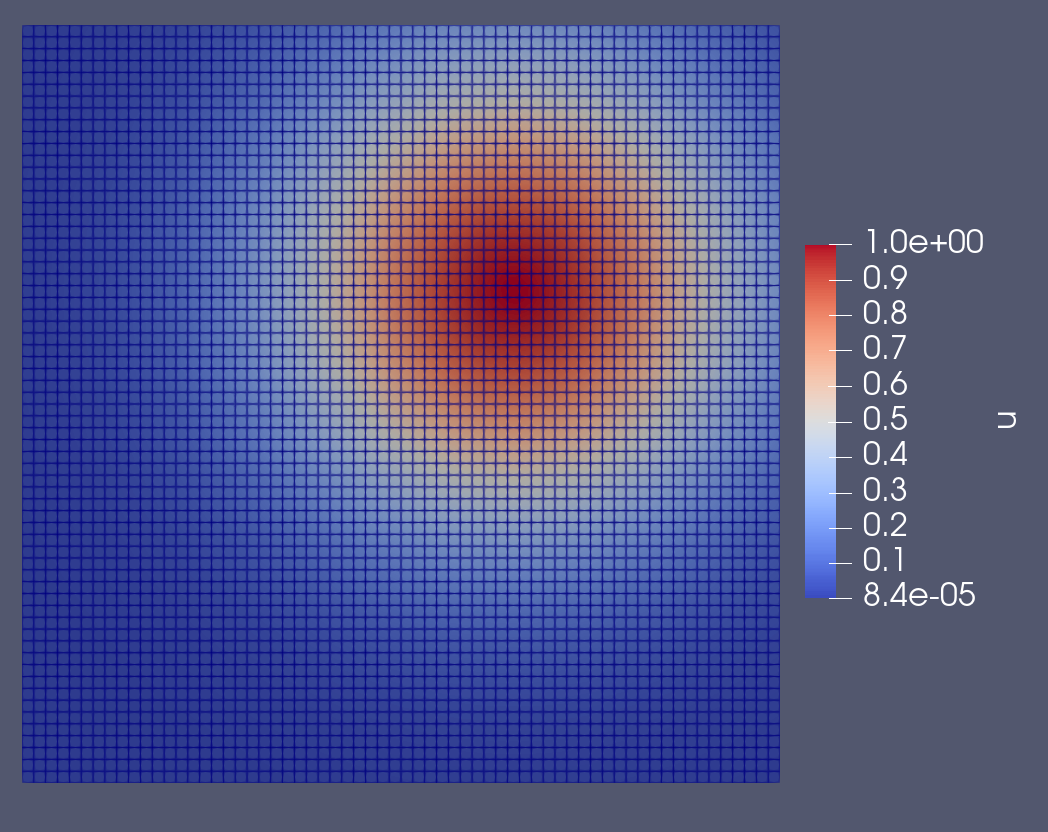
\includegraphics[width=10cm]{Figures/f1.png}
\vspace{-3.5mm}
\caption{Result for $\gamma = 0$}
\label{fig:rotProtocol}
\end{figure}

\textbf{5)} After runing the problem with FD jacobian, these are the results:

\begin{table}[h!]
\centering
\begin{tabular}{lcccc}
\hline
Jacobian & Relative error & Function eval & Final Residual & Time (s)\\
\hline
Analytical & $5.24\times10^{-4}$ & 2 & $6.38\times10^{-11}$ &  $1.107\times10^{-1}$ \\
FD (-snes\_fd) & $5.24\times10^{-4}$& 4228 &  $6.15\times10^{-11}$ &   $1.430$ \\
FD Colored (-snes\_fd\_color) & $5.24\times10^{-4}$& 7&  &  $1.174\times10^{-1}$  \\
\hline
\end{tabular}
\caption{Performance comparison for different Jacobian strategies.}
\label{tab:jacobian_full}
\end{table}

\textbf{6)}
\end{document}
